\newpage
\section{Componentenniveau}
In het componentenniveau worden het circuitniveau omgezet naar een component keuzes en schema's van de schakelingen. Dit wordt gedaan om het ontwerp van het circuitniveau om te zetten naar implementatie. 

\subsection{Temperatuur sensor}
In het circuitniveau is er gekozen voor een platina-weerstand. Hierin zijn er twee betaalbare varianten op de markt. De Pt1000 en Pt100. Het enige verschil is weerstandswaarde en de hoeveelheid stroom die er maximaal door de sensor mag lopen. De Pt100 heeft een weerstand van 100$\Omega$ en er mag maximaal 1,4 mA volgens de fabrikant en de Pt1000 heeft een weerstand van 1 k$\Omega$ en er mag maximaal 0.4 mA volgens de fabrikant \cite{Pt1000}. Doordat er een constante stroom door de sensor loopt, ontstaat zelfverwarming in de sensor. Dit maakt de sensor minder nauwkeurig. Om dit effect te verminderen, moet een zo laag mogelijke stroom door de sensor worden gestuurd via de stroombron. Om ervoor te zorgen dat het signaal van de sensor niet te klein wordt door de stroom te verlagen is er gekozen voor de Pt1000. Hierdoor kan de uitgang spanning net zo hoog blijven als bij de Pt100, maar dan met 10 keer minder stroom. Dit zorgt voor een lager energie verbruik. Voor het temperatuurbereik dat voor de applicatie nodig is. Gaat de weerstandswaarde variëren tussen de 980$\Omega$ en 1194$\Omega$ \cite{measure_tabel}.
\\
\newline
Om dit signaal te kunnen uitlezen is er een stroom bron nodig op een kleine stroom constant door de Pt1000 laat lopen. Uit het circuit niveau zijn de volgende eisen ontstaan voor de stroom bron.
\begin{itemize}
    \item Minimale SNR van 60 dB.
    \item Lage PPM om temperatuur om temperatuur onafhankelijk te zijn.
\end{itemize}
Naast deze eisen van het circuit niveau is er ook nog de eis vanuit het blokschema niveau waar maximaal 1 mW gebruikt mag worden door de sensor module. De sensor zelf is een passief component en gebruikt geen vermogen, maar de systemen om de Pt1000 uit te kunnen lezen wel. Door de sensormodule (stroombron plus Pt1000) op een lage voedingsspanning te laten werken, wordt het energieverbruik verlaagd. Daarom is gekozen voor een voedingsspanning van 3,3 volt. Bij lagere spanningen zijn er weinig opties voor versterkers en microcontrollers om de data te verwerken.
\\
\newline
Om ervoor te zorgen dat er een constante Stroom gaat lopen is er een referentie nodig waar de stroom aan gerefereerd kan worden. Deze referentie mag niet temperatuur gevoelig zijn en moet energie zuinig zijn. Uit onderzoek blijkt dat de ISL60002 serie van RENESAS voldoet aan deze eisen met een Stroom verbruik van 350 nA en PPM van 20 \cite{Spannings_ref}. Door deze spanningsreferentie met een transadmittantie versterker om te zetten naar een constante stroom ontstaat er een stabiele constante stroom die minimaal beïnvloed wordt door temperatuur verandering. Onder de voorwaarde dat de weerstand die hier voor gebruikt ook een lage ppm heeft. Dit idee is weergegeven in Figuur \ref{fig:transadmittantie_versterker}

\begin{figure}[H]
    \centering
    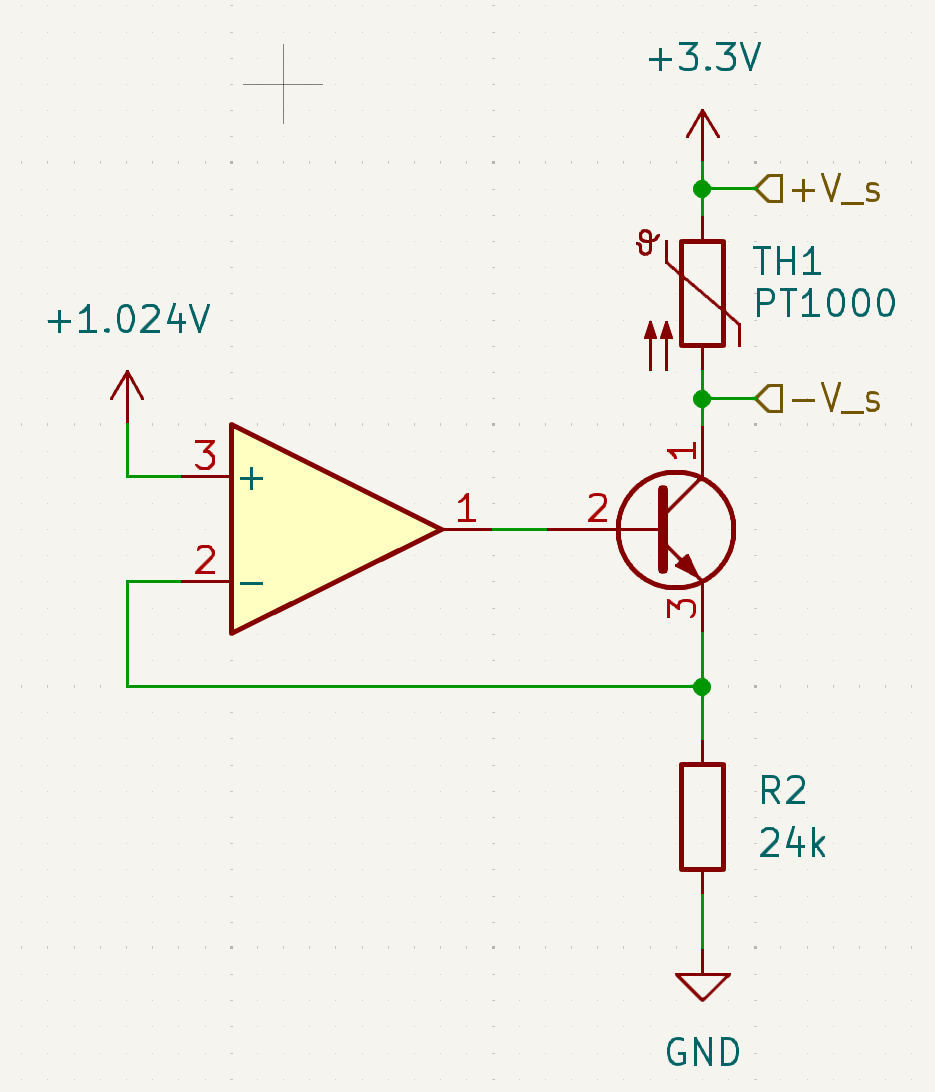
\includegraphics[width=0.5\linewidth]{pictures/Schema_current_source.png}
    \caption{De Pt1000 met een constante Stroombron.}
    \label{fig:transadmittantie_versterker}
\end{figure}

Door een weerstandswaarde van 24k$\Omega$ te plaatsen tussen de GND en de min ingang van de opamp en de emitter van de NPN-transistor. Zorg je ervoor dat de ingangsspanning door 24 duizend gedeeld wordt en er een constante stroom van 42,6$\mu$A loopt door de Pt1000. De grootste vermogensverbruiker is de opamp die gebruikt wordt in combinatie met de transistor om een nullor te creëren. Dit komt door de Quiescent stroom die een opamp minimaal nodig heeft om te kunnen functioneren. Om ervoor te zorgen dat er minder 1 mW aan vermogen verbruikt wordt door de sensor module moet er gekeken worden naar een opamp met een lage Quiescent stroom en lage maximale stroom verbruik. Met deze specificaties is er naar low power opamps gekeken. Hier kwam de LTC2055 \cite{LTC2055} met lage stroom verbruik het beste uit. Er is nog naar de MCP6002 \cite{MCP6002} gekeken, deze is minder zuinig, maar qua prijs goedkoper. De LTC2055 is gekozen vanwege het lagere energieverbruik en de lagere maximale stroom. Als laatste moet er een keuze worden gemaakt voor het type NPN-transistor dat gebruikt moet worden. Omdat de opamp zijn parameters richting nul gaan heeft de ruis van de Transistor weinig tot geen invloed op de schakeling en is deze daarom te verwaarlozen. Hierom is er gekozen voor de NPN-transistor die al aanwezig was op school tijdens het project. Er is daarom gekozen voor de B547 \cite{B547} dit bespaart kosten, omdat deze transistor niet extern ingekocht hoeft te worden.
\\
\newline
Nu de componenten zijn gekozen op basis van hun lage verbruik en prestaties, is het belangrijk om de nauwkeurigheid van deze specifieke stroombron verder te analyseren door te kijken naar de ruisbijdragen in de schakeling. De ruis in dit systeem kan de precisie van de stroombron beïnvloeden, dus bespreken we in de volgende sectie de verschillende ruisbronnen en hun kwantitatieve bijdragen. Hierbij richten we ons op de \(1/f\)-ruis en witte ruis van de spanningsreferentie en opamp, evenals de thermische ruis van de weerstand.
\\
\newline
Door deze ruisbijdragen samen te nemen, kunnen we de totale stroomruis berekenen en zo inzicht krijgen in de nauwkeurigheid van de stroombron.

\subsubsection{Ruis berekening van de Stroombron}
Om de nauwkeurigheid van de stroombron te kwantificeren, berekenen we hieronder de bijdragen van de verschillende ruisbronnen:

\begin{enumerate}
    \item \textbf{Ruis van de spanningsreferentie} \\
    De spanningsreferentie genereert \(1/f\)-ruis, die onder een cutoff-frequentie van 10 Hz dominant is, en een constante witte ruis daarboven. De \(1/f\)-ruis wordt berekend met de volgende formule:
    \[
    U_{n,\text{ref, flicker}} = A_{\text{ref}} \cdot \ln\left(\frac{f_{\text{cutoff}}}{f_{\text{low}}}\right)
    \]
    waarbij \(A_{\text{ref}}\) afhankelijk is van de witte ruis boven de cutoff-frequentie. De uitkomst geeft de ruis van de spanningsreferentie die de stabiliteit van de stroombron kan beïnvloeden.

    \item \textbf{Ruis van de opamp} \\
    De opamp heeft een vergelijkbare ruisbijdrage als de spanningsreferentie, met \(1/f\)-ruis onder een cutoff-frequentie van 10 Hz en witte ruis daarboven. Op dezelfde manier wordt de \(1/f\)-ruis van de opamp als volgt berekend:
    \[
    U_{n,\text{opamp, flicker}} = A_{\text{opamp}} \cdot \ln\left(\frac{f_{\text{cutoff}}}{f_{\text{low}}}\right)
    \]
    waarna deze spanningsruis wordt omgezet naar stroomruis om het effect op de uitgangsstroom van de stroombron in te schatten.

    \item \textbf{Thermische ruis van de weerstand} \\
    De thermische ruis van de weerstand wordt berekend met de formule:
    \[
    I_{n,\text{resistor}} = \sqrt{\frac{4 k_B T}{R}}
    \]

    \item \textbf{Spanningsruis omzetten naar stroomruis}
    De spanningsruis van de opamp en spanningsreferentie kunnen worden omgezet naar stroomruis door de weerstand. Dit wordt berekend met de formule:
    \[
    I_{n}^2 = \frac{U_{n}}{R^2}
    \]

    \item \textbf{Totale stroomruis} \\
    De totale stroomruis van de stroombron wordt berekend als de kwadratische som van de stroomruiscomponenten:
    \[
    I_{n,\text{total}} = \sqrt{I_{n,\text{ref}}^2 + I_{n,\text{opamp}}^2 + I_{n,\text{resistor}}^2}
    \]
    Dit geeft ons de uiteindelijke ruisbijdrage die de precisie van de stroombron bepaalt en de stabiliteit van het systeem beïnvloedt. Door deze formules in te vullen voor de gewenste bandbreedte van 0,1 tot 1 Hz resulteert dit in de volgende formule:
    \[
    I_{n,\text{total}} = \sqrt{(1,9188 \cdot 10^{-9})^2 + (1,7269 \cdot 10^{-10})^2 + (8,6877 \cdot 10^{-13})^2} = 1,9266 \cdot 10^{-9}\; \text{A}
    \]

    \item \textbf{Signaal ruis verhouding}
    Met de berekende stroomruis is het nu mogelijk om de SNR van de stroombron te berekenen. Dit is weergegeven in de volgende formule:
    \[
    \text{SNR} = 20log(\frac{4,26 \cdot 10^{-5}}{1,9266 \cdot 10^{-9}} = 86.906\; \text{dB}
    \]
\end{enumerate}
Nu berekend is dat de Stroombron voldoet aan de SNR-specificatie is het belangrijk om te berekenen hoeveel vermogen het systeem gaat gebruiken. Hiervoor wordt de informatie uit de datasheets gebruikt voor stroomverbruik. Dit is weergegeven in de volgende formule:
\[
P_{totaal} = \alpha \cdot \frac{T}{T_actief} \cdot P_{actief} + (1-\alpha \cdot \frac{T}{T_actief}) \cdot P_{lek}
\]
Omdat er altijd een constante stroom door de Pt1000 moet lopen is er geen $P_{lek}$ dit zorgt ervoor dat de formule versimpeld kan worden naar de volgende formule.
\[
P_{totaal} = P_{actief}
\]
Door deze formule in te vullen door informatie van de datasheets \cite{LTC2055,Spannings_ref} zorgt ervoor dat de geschatte vermogens verbruik rond de 0,5 mW wat is weergeven in de volgende Formule:
\[
P_{\text{}} = 3,3 \cdot 150 \cdot 10^{-6} + 5 \cdot 350 \cdot 10^{-9} = 0,496 \; mW
\]

\subsection{Luchtvochtigheid sensor}
% SHT45


\subsection{Digitale bewerking}
%ADC, MCU, DAC
benodigdheden zijn: i2c voor uitlezen luchtvochtigheid, adc voor uitlezen temp sensor, gpio pin voor aansturen zender, gpio pin voor aan uit schakelen zender en versterker ivm stroom verbruik. sleep modus voor verlagen stroom verbruik.
attiny1624, heeft alles en weinig extra, enige extra zijn een aantal communicatie protocollen als spi en uart, maar dat is bijna altijd als er een protocol als i2c nodig is.
power down modus waarbij stroomverbruik enkele $\mu$A is. daarbij draait alleen nog de RTC op de ingebouwde 32 kHz oscillator, de rest staat allemaal uit. De RTC kan gebruikt worden om uit de power down modus te komen. In de Specificaties is aangeven dat er minimaal elke 10 seconde nieuwe data verstuurd moet worden. De RTC kan gebruikt worden om elke 8 seconde een interrupt te maken en er zo dus elke 8 seconde een meting gedaan kan worden.
Voedingsspanning van 3.3 volt voor minder verbruik, goed voor 5MHz klok om zo snel mogelijk data te verwerken en te versturen en in verhouding zo lang mogelijk in de zuinige slaap modes te zijn. 



\subsection{Instrumentatie versterker}
De stroom die door de Pt1000 loopt zorgt ervoor dat er over de Pt1000 een spanning gaat staan in de mV. Om dit signaal te kunnen verwerken in het digitale domein is het nodig om deze spanning te versterken. In het circuit niveau is bepaald dat dit gedaan moet worden door middel van een instrumentatie versterker. Het uitgangssignaal van de Pt1000 gaat variëren tussen de 41,81 en 50,94 mV. Dit zorgt voor een dynamisch bereik van 9,13 mV en een statisch signaal van 41,81 mV. Het digitale systeem een ADC van 12 bit. Dit zorgt ervoor dat er over het bereik van de ADC 4096 stappen zijn. Met deze specificatie ontstaat er een LSB van 0,805 mV. Hierdoor is het nodig dat het signaal van de Pt1000 minimaal versterkt wordt naar een signaal waar het temperatuurverschil zichtbaar is in LSB. Uit de volgende Formules komt het resultaat uit dat er een minimale versterking van 105,8 nodig is om de specificaties van de ADC te bereiken.
\[
\frac{\frac{V_{dynamisch}}{Minimale\; ADC\; stappen}}{LSB} \cdot A = 1
\]
\\
\[
\frac{\frac{9,13 mV}{1200}}{0,805 mV} \cdot A = 1
\]
Door de formule te herschrijven zodat A geïsoleerd is resulteert dat in de volgende formule
\[
A = \frac{1}{\frac{\frac{9,13 mV}{1200}}{0,805 mV}} \geq 105,8
\]
Als deze versterking in één keer plaats vind, wordt het signaal op de uitgang van de Instrumentatie versterker 5,389 V dit gaat boven de voedingsspanning van het systeem. Hierom moet de versterking in twee trappen gedaan waar tussen een deel van het statische signaal weg gehaald wordt om ervoor te zorgen dat het signaal binnen de voedingsspanning blijft. Zoals is weergegeven in Figuur \ref{fig:schema_versterkers_component_1}.

\begin{figure}[H]
    \centering
    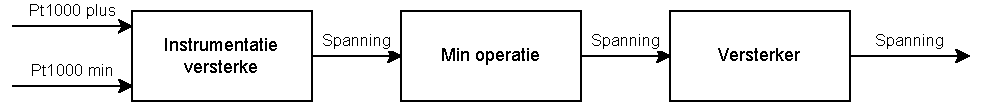
\includegraphics[width=0.8\linewidth]{pictures/schema_instrumentatie_versterker.drawio.pdf}
    \caption{Schematische weergave van de versterker implementatie.}
    \label{fig:schema_versterkers_component_1}
\end{figure}

Om de ruis van de tweede versterker en min operatie zo min mogelijk invloed te laten hebben op het SNR is het nodig dat de Instrumentatie versterker zo veel mogelijk versterkt. Een versterking van 53 keer zo hiervoor het beste uitkomen, doordat het halverwege het doel zit van de minimale versterking die nodig is om de eisen van de ADC te halen. Met daarbij zorgt een versterking van 53 keer voor een maximaal signaal van 2,69 Volt en minimaal signaal van 2,21 Volt. Deze signalen zitten binnen de voedingsspanningen. Door met de min operatie er minimaal 1,1 volt van af te halen kan daarna het signaal versterker worden met een factor 2 om de beoogde signaalgrootte te behalen.
\\
\newline
Door een grotere spanning van het signaal af te halen met de min operator is het mogelijk om het uitgangssignaal meer in het midden van het ADC bereik te plaatsen. Dit wordt gedaan om ervoor te zorgen dat het signaal meer in het lineaire gebied van de ADC te plaatsen wat het trimmen van de informatie makkelijker maakt. Door deze reden is er gekozen voor een spanning van 2 Volt. Hierdoor komt er op de ingang van de versterker een signaal tussen de 0,21 Volt en 0,69 Volt. Dit resulteert dan in een spanning tussen de 0,42 Volt en 1,389 Volt. Dit is niet in het midden van de ADC. Om hiervoor te zorgen is het nodig om het signaal meer te versterken. Hierom is er gekozen voor een versterking van 4. Dit zorgt ervoor dat de resolutie van de ADC per 0.1 $^\circ\text{C}$ hoger is dan de opgestelde specificatie. Dit maakt het makkelijker om het signaal te trimmen en kalibreren.
\\
\newline
De min operatie en versterkingstrap kan worden samengevoegd door het gebruik van een tweede Instrumentatie versterker. Dit zorgt voor versimpeling in het circuit. Dit resulteert in de volgende schema weergegeven in figuur \ref{fig:schema_versterkers_component_2}.

\begin{figure}[H]
    \centering
    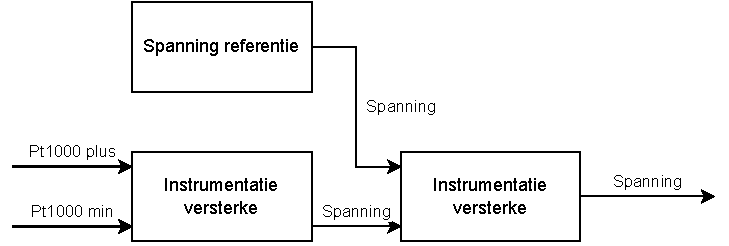
\includegraphics[width=0.8\linewidth]{pictures/schema_instrumentatie_versterker_1.drawio.pdf}
    \caption{Schematische weergave van de versterker implementatie.}
    \label{fig:schema_versterkers_component_2}
\end{figure}

De keuze voor de specifieke Instrumentatie versterker implementatie bepaalt het vermogensverbruik. Uit onderzoek blijkt dat het meer vermogen kost om de Instrumentatie versterker op te bouwen met meerdere versterker in vergelijking tot IC waar de volledige Instrumentatie versterker in zit op de terugkoppelweerstand na. Voor deze reden wat er gekeken naar verschillende Instrumentatie versterker IC's. In de weergegeven Tabel worden verschillende IC vergeleken \ref{tab:amplifer_comparison} met informatie uit de datasheets \cite{AD8220, AD8226, INA828}.

\begin{table}[H]
    \centering
    \begin{tabular}{|c|c|c|c|c|c|c|}
        \hline
        \textbf{Versterker} & $V_{Operating}$ & $I_{Quiescent}$ & $V_{input}$ & $V_{output}$ & $V_{ruis}$ & $I_{ruis}$ \\ \hline
        
        \textbf{AD8220} &  4,5 - 36 &  750$\mu$ & 0 - $V_s$-2,2 & 0,2 - $V_s$-0,2 & $14 nV\sqrt{Hz}$ & $1 fA\sqrt{Hz}$ \\ \hline
        
        \textbf{AD8226} & 2,2 - 36 & 425$\mu$ & 0 - $V_S$ & 0,1 - $V_s$-0,1 & $22 nV\sqrt{Hz}$ & $100 fA\sqrt{Hz}$\\ \hline
        
        \textbf{INA828} & 4,5 - 36 & 600$\mu$ & 2 - $V_s$-2 & 0,15 - $V_s$-0.15 & $7 nV\sqrt{Hz}$ & $170 fA\sqrt{Hz}$\\ \hline
        
    \end{tabular}
    \caption{Vergelijking verschillende versterkers.}
    \label{tab:amplifer_comparison}
\end{table}
Voor het voeden van deze IC wordt een andere spanning gebruikt dan de rest van het systeem. Dit wordt gedaan om deze versterkers meer overhead te geven. Hierom is gekozen voor een voedingsspanning van 5 Volt. Met deze spanning kan alle drie de optie gevoed worden. Uit de Tabel \ref{tab:amplifer_comparison} en datasheet is te zien dat de INA828 niet gebruikt kan worden door het kleine ingang spanning bereik. Dit zou opgelost kunnen worden door een nog hogere voegingsspanning te nemen. Dit zorgt voor meer vermogen verbruik en is daarom ook niet voor gekozen. Dan blijven de AD8220 en AD8226 over waar de AD8226 zuiniger is ten koste van een hogere ruis. Dit komt doordat de AD8220 jfet's gebruikt aan de ingang om de ruis te beperken, dit zorgt dan weer wel voor een hogere $I_{Quiescent}$. Daarnaast heeft de AD8220 net zoals de INA828 een beperkt input bereik aan de bovenkant. Dit zorgt ook voor problemen doordat het ingangssignaal van de Instrumentatie versterker tussen de 3,3 Volt en 3,25 Volt ligt. Zoals is weergegeven in Figuur \ref{fig:transadmittantie_versterker}. Hierdoor kan de AD8220 het signaal niet goed verwerken. Zonder de voedingsspanning, wat nog een optie kan zijn als de AD8226 te veel ruis genereert. 

\subsubsection{Ruis berekeningen van de Instrumentatie versterker}
De Ruis berekeningen voor de versterker zijn gedaan in Octave hierdoor is het simpel om de twee opamp te vergelijken. De code die gebruikt voor deze berekeningen is te vinden in de bijlages~\ref{lst:octave_code_noise},~\ref{lst:octave_code_noise_current}. Uit deze berekeningen blijken de volgende waardes voor SNR van beide opamps. Zoals is weergegeven in Tabel \ref{tab:SNR_opamps}.

\begin{table}[H]
    \centering
    \begin{tabular}{|c|c|}
        \hline
         \textbf{Versterker} & \textbf{SNR} \\ \hline
         AD8220 & 72,2808 dB \\ \hline
         AD8226 & 72,3018 dB \\ \hline
    \end{tabular}
    \caption{SNR van de twee mogelijke versterkers.}
    \label{tab:SNR_opamps}
\end{table}
Uit de berekening blijkt dat de AD8226 zelfs beter presteert, dit komt doordat de AD8220 een hogere \(1/f\)-ruis heeft. Deze ruis overheerst de ruis in het laag frequent gebied waar de Pt1000 in werkt het meeste. Vanwege deze reden is er gekozen voor de AD8226. De spectrale ruis is weergegeven in Figuur \ref{fig:spectral_ruis_plot}.

\begin{figure}[H]
    \centering
    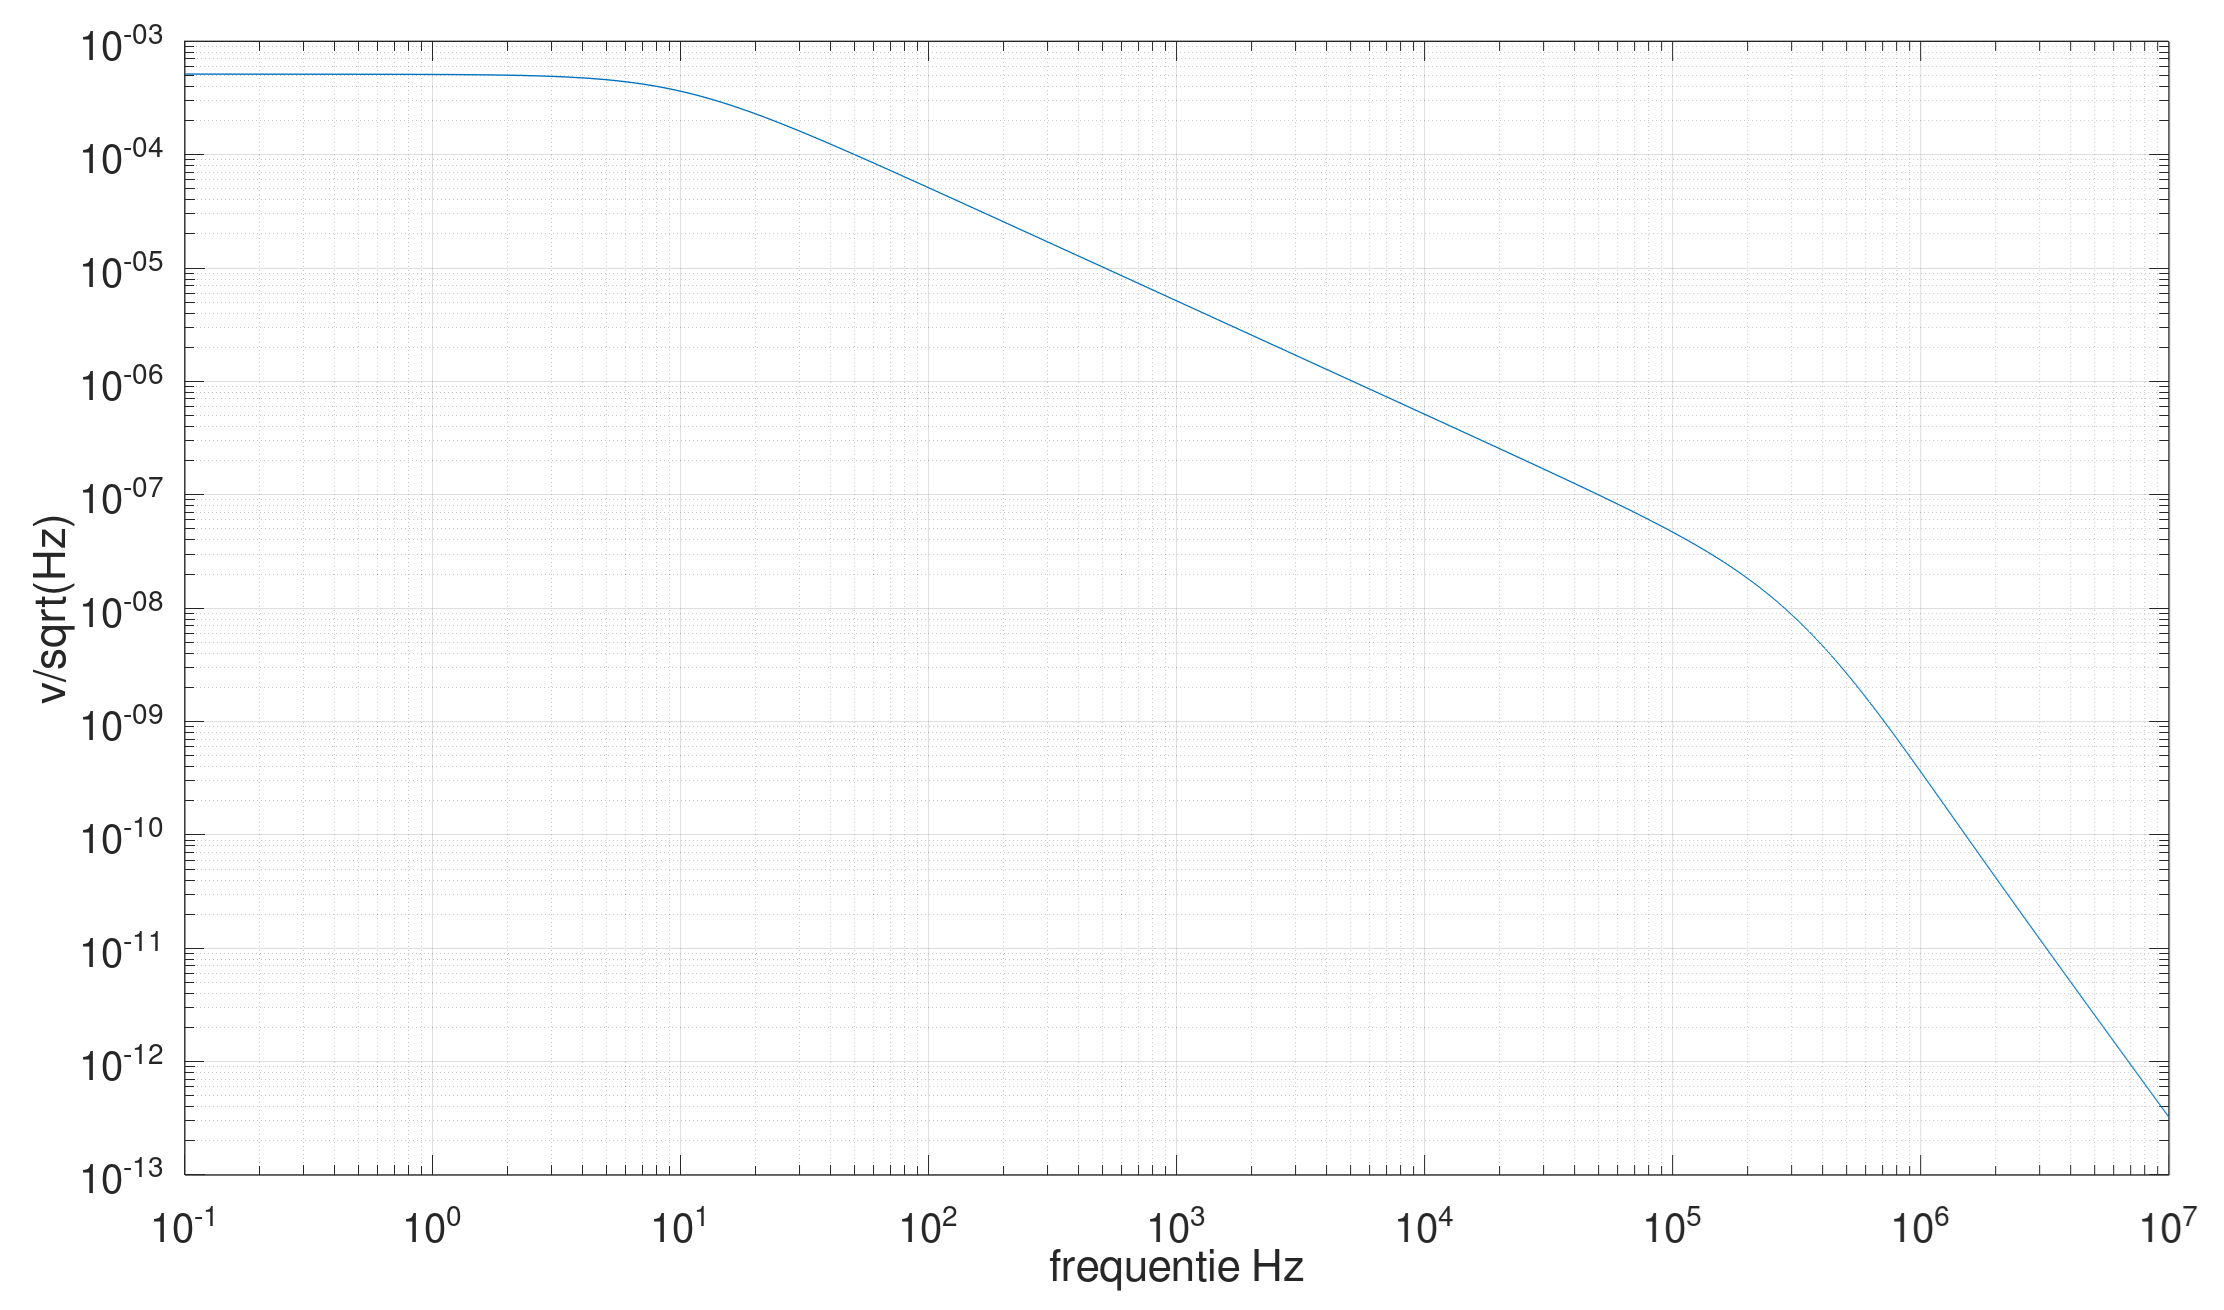
\includegraphics[width=0.9\linewidth]{pictures/ruis_plot.png}
    \caption{Spectrale ruis van de Temperatuur sensor over een frequentie bereik van 0,1 Hz tot 10 MHz.}
    \label{fig:spectral_ruis_plot}
\end{figure}

Door het verbruik van de AD8226 van 400 $\mu$A per opamp is het nodig om de versterkers uit te kunnen zetten. Om te voldoen aan de richtlijn van het energieverbruik die zijn opgesteld in de paragraaf \ref{Block_schema}: Blokschema niveau. Zonder de Versterkers uit te zetten wordt er een minimaal vermogen van 2 mW door de $I_{Quiescent}$. Dit kan beperkt worden een schakelaar in de voedingslijn te plaatsen die door de microcontroller bepaald kan worden. Dit zorgt ervoor dat de versterkers alleen aan staan als de er gemeten moet worden. Hierdoor is het mogelijk om het energieverbruik te verlagen van minimaal 2 mW naar 65 $\mu$W. Dit komt door dat de sensor lang in rust modus staat en maar heel kort data aan het verwerken is op de microcontroller. Deze schakelaar kan gerealiseerd worden door een N-channel mosfet te plaatsen in voedingslijn tussen GND en de minvoedingspin van de AD8226. Dit is weergegeven in Figuur \ref{fig:Instrumentatie_amp_schematic}.
Met deze aanpassing is het vermogensverbruik onder de richtlijn en zorgt dit ervoor dat er meer vermogen ergens anders gebruikt kan worden. 
\begin{figure}[H]
    \centering
    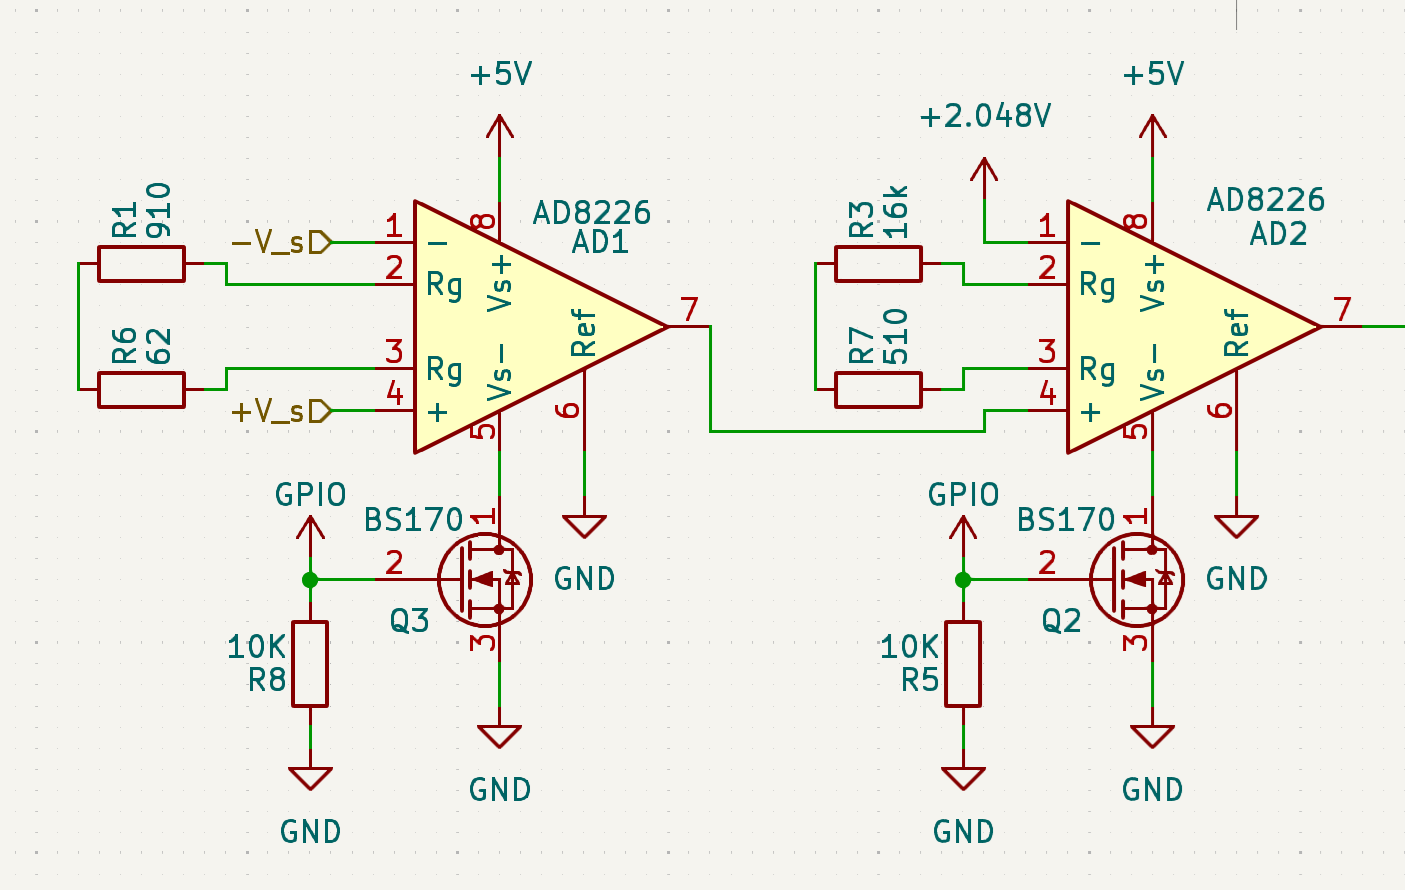
\includegraphics[width=0.7\linewidth]{pictures/Intrumentatie_amplifier_schematic.png}
    \caption{Schematische weergave van Instrumentatie versterker opbouw.}
    \label{fig:Instrumentatie_amp_schematic}
\end{figure}

\subsection{Anti aliasing filter}
Het signaal dat door van de Pt1000 door de instrumentatie versterker wordt geleverd aan de ADC. Dit signaal kan door EMC en storing verstoord worden in hoge frequentie gebied. Om dit te minimaliseren is een anti aliasing filter nodig dat deze frequentie wegdempt. Dit wordt gedaan door een enkele orde Butterworth die een kantelpunt heeft van 10 Hz. Hierdoor wordt de informatie van de Pt1000 niet vervormd door het filter en worden hogere frequentie weg gedempt. Na de anti aliasing filter is een opamp geplaatst als buffer om te voorkomen dat de ADC het filter gaat beïnvloeden. Nu met dit filter is het mogelijk om de volledige Temperatuur sensor te gaan opbouwen en testen. In Figuur \ref{fig:complete_temp_sensor} is het volledige schema weergegeven.
\begin{figure}[H]
    \centering
    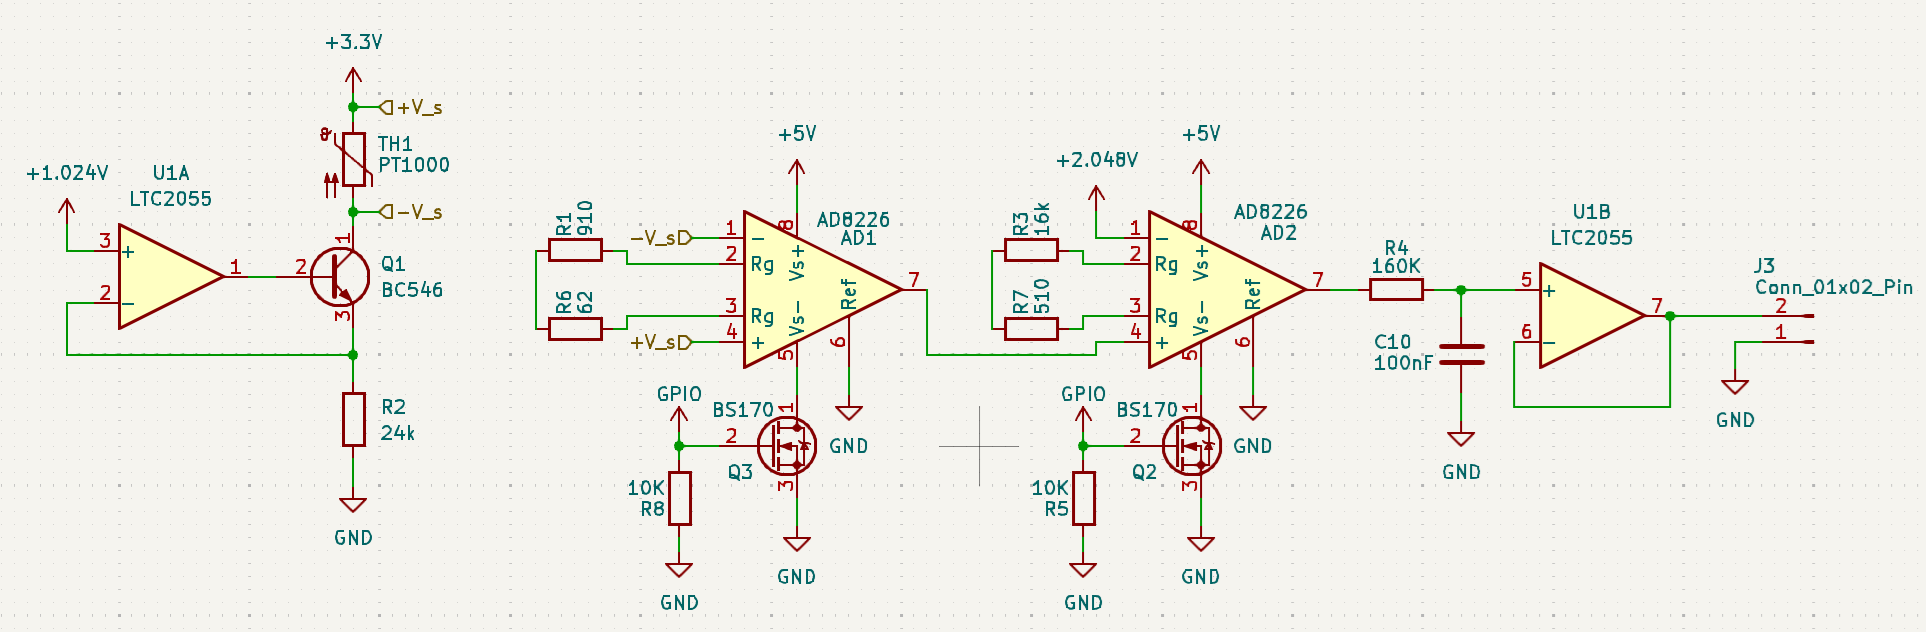
\includegraphics[width=1\linewidth]{pictures/Temp_sensor_complete_schematic.png}
    \caption{Volledig schema voor de temperatuur sensor tot aan de ADC.}
    \label{fig:complete_temp_sensor}
\end{figure}

% dan de versterker uitleggen
% plus ruis

% keuzes uitleggen en berekening energie verbruik


\newpage
\subsection{Zender}